\subsection{Técnicas de Questionario}
	Técnicas de questionario são aplicadas em testes de usabilidade em que há participação do usuario, com o objetivo de descobrir se o software esta suprindo as necessidades e expectativas do usuario.

	Na maioria das vezes, um modelo de questionário apóia-se nas experiências e
	heurísticas de seus elaboradores. Quando é utilizado em pesquisas reais ou simuladas, o
	modelo depara-se com circunstâncias e necessidades não previstas inicialmente, o que
	determinará os refinamentos e ajustes, que, aplicados sucessivamente, permitirão a
	evolução das questões ~\cite{usabilidade_web}. 
	
	As técnicas são úteis para se obter detalhes que, do ponto de vista dos desenvolvedores, não são observados.Estes detalhes são utilizados para obter informações relativas as necessidades dos usuários e revelar possíveis problemas que nós, desenvolvedores, normalmente nao veríamos.
	
	Serão realizados questionarios afim de se obter dados quantitativos, o questionario também possui a vantagem de atingir um número maior de usuarios, o que facilita ainda mais a coleta de dados relevantes a respeito da Interação Humano-Computador do sistema Enturma.
	
	


\subsection{Avaliação de Usabilidade e Questionario de Satisfação dos Usuários}

	A avaliação da usabilidade será realizada com a utilização do software Enturma, facilitando o registro de problemas encontrados durante a utilização do sistema pelos usuários da aplicação.
	
	A proposta do questionario a ser aplicado aos usuários após a realização da avaliação de usabilidade com base no \textit{WAMMI} (\textit{Website Analysis and MeasurMent Inventory}) e no \textit{QUIS} (\textit{Questionnaire for User Interactional Satisfaction}).


	O \textit{QUIS} é uma ferramenta que foi desenvolvida por pesquisadores do \textit{Human Computer Interaction Laboratory (HCIL)} da \textit{University of Maryland}, para medir a satisfação do usuário, focando em objetivos especificos da Interação Humano-Computador.
	
	As questões são apresentadas na forma de afirmações
utilizando as escalas de diferencial semântico, que
baseiam-se em explorar uma faixa de atitudes bipolares
representada por um par de adjetivos. As questões são
respondidas em uma escala que varia de O a 9, onde o zero
representa um adjetivo negativo e os demais representam
adjetivos positivos. Por ser um questionário geral utilizado
para uma ampla variedade de produtos, também inclui a
opção N/A (não-aplicável). A Tabela \ref{tab:exemploQuestao} mostra um exemplo
de uma questão com escalas de satisfação específica. ( Filardi; Traina, 2008)

\begin{table}[H]
	{Exemplo de uma questão de QUIS utilizando escala de diferencial semantico}
	\centering
	\begin{tabular}{|c|c|c|c|c|c|c|c|c|c|c|c|c|c|c|} 

		\hline
		   QUIS &  & 1 & 2 & 3 & 4 & 5 & 6 & 7 & 8 & 9 & N/A &  \\
		\hline
		Mensagens que aparecem na tela & Confusa &  &  &  &  &  &  &  &  &  &  & clara \\ 

		\hline
	\end{tabular}
	\caption {Fonte:Filardi; Traina, 2008}
	\label{tab:exemploQuestao}

\end{table}

	O \textit{WAMMI} é um serviço exclusivo para avaliação de
\textit{Websites on-Iine}, com o propósito de ajudar os proprietários
do site a cumprir suas metas corporativas através da
medição e monitoramento das reações do usuário sobre
suafacilidade de uso. Através de um botão colocado no site,
é disponibilizado um questionário com a estrutura de um
formulário para ser preenchido. Os dados do questionário
são armazenados e analisados a partir de uma base de dados
padronizada com \textit{escores} normalizados. São utilizados para
avaliar os seguintes aspectos: atratividade, controle,
eficiência, utilidade, aprendizagem e usabilidade global.
	
	O \textit{WAMMI} tem como objetivo: 

\begin{itemize}
	\item medir a satisfação do usuário sobre o site baseado na
reação do usuário;
	\item gerar dados objetivos de gestão em um formato fácil de
entender;
	\item prover uma base para mudanças do Website e melhorias
de design;
	\item comparar seu site em relação aos demais em termos de
satisfação do usuário; 
	\item acompanhar o desempenho do Website para verificar se
as metas estão sendo cumpridas.
\end{itemize}

Fonte:Filardi; Traina, 2008

\subsection{Roteiro de Utilização do Sistema} % (fold)
\label{sub:roteiro_de_utiliza_o_do_sistema}
	
	Com o objetivo de obter informação suficiente para garantir que todos as funcionaliades do sistema foram avaliadas, foi desenvolvido um roteiro ao qual o usuário deverá seguir no momento em que for utilizar o sistema Enturma.

	O sistema Enturma possui 3 (três) Casos de Uso, e com objetivo de avaliar todos os Casos de Uso, foram desenvolvidos roteiros específicos para cada Caso de Uso, como pode ser observado a seguir.


	\begin{enumerate}
		\item \textbf{Visualizar Rankings}:

			Para conclusão do roteiro de visualização dos Rankings, o usuário deverá:

				\textbf{-} Acessar o sistema Enturma (www.projetoenturma.com.br);
				
				\textbf{-} Acessar a seção de Serviços;
				
				\textbf{-} Selecionar Ranking;
				
				\textbf{-} Selecionar a turma desejada;
				
				\textbf{-} Visualizar todos os tipos de Ranking disponíveis.

		\item \textbf{Acompanhar Turma}:
			
			Para conclusão do roteiro de Acompanhamento de Turmas, o usuário deverá:
				
				\textbf{-} Acessar o sistema Enturma (www.projetoenturma.com.br);
				
				\textbf{-} Acessar a seção de Serviços;
				
				\textbf{-} Selecionar a opção de Relatórios de Turmas;
				
				\textbf{-} Selecionar a turma desejada e seus filtros;
				
				\textbf{-} Visualizar todos os dados obtidos;
				
				\textbf{-} Limpar a pesquisa para a realização de uma nova pesquisa.

		\item \textbf{Comparar Turmas}:

			Para conclusão do roteiro de Comparação entre Turmas, o usuário deverá:
				
				\textbf{-} Acessar o sistema Enturma (www.projetoenturma.com.br);
				
				\textbf{-} Acessar a seção de Serviços;
				
				\textbf{-} Selecionar Comparar Turmas;
				
				\textbf{-} Selecionar as duas turmas e seus filtros;
				
				\textbf{-} Visualizar os dados obtidos;
				
				\textbf{-} Limpar pesquisar para realização de uma nova pesquisa.

	\end{enumerate}
% subsection roteiro_de_utiliza_o_do_sistema (end)

\subsection{Verificação da Interface Gráfica} % (fold)
\label{sub:verifica_o_da_interface_gr_fica}

	Com o objetivo de Verificar a qualidade da Interface Gráfica, utilizaremos a ferramenta ASES, que é um software desenvolvido pelo Governo Federal com o objetivo de Avaliar o nível de Acessibilidade em sistemas web. O software faz uma verificação em todas as páginas do sistema e aponta erros e avisos que não seguem o padrão e-Mag.

	O sistema pode ser observado na imagem a seguir e os resultados obtidos estão dispostos na seção de Análise dos Resultados.

	\begin{figure}[H]
		\centering
		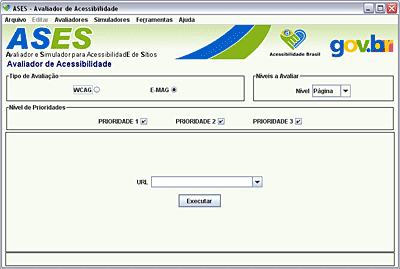
\includegraphics[width=0.7\textwidth]{imagens/ASES}
		\caption{Avaliador e Simulador de AcessibilidadE de Sítios}
		\label{img:ASES}
	\end{figure}
% subsection verifica_o_da_interface_gr_fica (end)